

\chapter{Tests and Results}
\label{ch:evaluate}

In the previous chapter, the implementation of the secondary structure logic in HMModeler was described. In the following chapter, the changes made to HMModeler will be evaluated by testing the different scoring and weighting methods that were used.

All test datasets and the database, as well as the generated scores and plots mentioned in the following chapter, can be found on the attached disk (see Appendix \ref{app:AppDisk}).

\section{Test Dataset}
\label{sec:TestData}


 The ASTRAL SCOP 1.73 sequence database\footnote{Astral SCOP 1.73: \url{https://scop.berkeley.edu/astral/ver=1.73} (accessed July 18, 2018).}, filtered to retain entries  with less than 40\,\% sequence similarity to each other, was used. This specific version was chosen because it was the latest complete manually curated version available at the time of writing this thesis.  
 The database contains 9,536 sequences with an average sequence length of 178 residues. While most residues in the database are from the 20 common amino acids listed in Table \ref{tab:AAlist}, 452 are ambiguous residues. Apart from one, these ambiguous residues are all defined as \textit{any of the 20 common amino acid residues} and represented by the letter X. 
 As described in Section \ref{sec:inputData}, the logic for sequences with the symbol X is implemented for both the primary and secondary structure. The single additional ambiguous residue, marked by the symbol Z, occurs in the sequence with the \ac{SID} \texttt{d4cpai\_}, representing a position with either glutamine (Q) or glutamic acid (E).  This sequence was removed from the database, as these rare special cases would lead to an extensive expansion of the implementation, such as an additional emission case for each possible ambiguous amino acid. Furthermore, this would also lead to an increased \mbox{run-time} of the training and scoring algorithms.  
 Another approach to handle ambiguous amino acids is, as described in \mbox{\cite[p.~183]{Baldi.2001}}, ``the  `benefit of the doubt'    approach'', where ambiguous amino acids are replaced with the most likely candidates for these positions.  
 With the sequence containing the symbol Z removed from the database, the test set finally contained 9,535 sequences. As each entry listed in \ac{SCOP} is linked to \mbox{three-dimensional} structure information in the \ac{PDB}, the secondary structure for the test set was determined using DSSP.  
 
A set of 69 \acp{MSA} based on the  same ASTRAL \ac{SCOP} 1.73 database was provided by the Department of Molecular Biology at the University of Salzburg\footnote{University of Salzburg: Department of Molecular Biology: \url{https://biwww.che.sbg.ac.at/} (accessed July 18, 2018).}. Each MSA is built up from 15 homologous sequences within  the same superfamily. 
For the first tests of the scoring and weighting methods of the \ac{pHMM}, the secondary structure from \ac{DSSP} was also used for the \ac{MSA}, as it represents the perfect condition in combination with the used test database assigned the same way. 

For the first part of the following section, the \ac{MSA} representing the \ac{SCOP} superfamily \texttt{c.67.1} will mainly be used in order to show changes in the score types when including secondary structure. 
The superfamily \texttt{c.67.1} is from the class \textit{alpha and beta proteins (a/b)} and represents \textit{pyridoxal phosphate-dependent transferase} proteins that are involved in the biosynthesis of amino acids dependent on \textit{pyridoxal phosphate}. This is the active form of vitamin B6.  
The \ac{MSA} with 15 sequences is 501 columns long. The \acp{pHMM} trained from the \ac{MSA} have a length of 384 match-states. 
More than 50\,\% of the remaining 116 columns consist of gaps and thus are represented as insertion states in the \ac{pHMM}. 
In total, the \ac{MSA} includes 5,966 residues and 1,549 gap positions.
The complete \ac{MSA} \texttt{c.67.1} in its Stockholm format is provided in Appendix \ref{app:MSAc671}. 
In the SCOP database that was used, 60 out of the 9,535 sequences are classified as belonging to the superfamily \texttt{c.67.1}.

The secondary structure for the 15 sequences of the \ac{MSA} was assigned by DSSP, using the associated structure files in the \ac{PDB}. 
The class \textit{alpha and beta proteins (a/b)}, to which the \ac{MSA} belongs, is structurally composed of alternating alpha helices and beta sheets in which the beta sheets are mostly parallel to each other. Therefore,  the \ac{MSA} is represented by a balanced number of all three secondary structure elements.
Table \ref{tab:SSdist} lists the number of occurrences and the percentage distribution of the secondary structure classes assigned by \ac{DSSP}  for the  database that was used and the \ac{MSA} \texttt{c.67.1}. The data show that in general, loops are the most common structure with 43.1\,\%, followed by helices, and finally sheets, which are the least common. 

\begin{table}[h]
\centering
\begin{tabular}{|l|rr|rr|} 
\hline
SS-Class 		& 	& SCOP 1.73			&  	& \ac{MSA} c.67.1 \\ \hline
Helix H 		& 35.1\,\%	& 594,399 		& 41.9\,\% 	& 2,497   \\
Sheet E 		& 21.8\,\%	& 368,469 		& 16.6\,\%	& 991    \\ 
Loop \,C 		& 43.1\,\%	& 729,494 		& 41.4\,\%	& 2,472   \\
Any \ \ X 		& $<0.1$\,\%	& 451    		& 0.1\,\%	& 6     	\\ \hline
Total 	&100 \% 	& \qquad 1,692,815 	& 100  \%	& \qquad 5.966 \\ \hline 
\end{tabular}
\caption[Distribution of the secondary structure elements.]{Distribution of the secondary structure elements $H$, $E$,  $C$ and $X$ in the SCOP database and the \acs{MSA} c.67.1.}
\label{tab:SSdist}
\end{table}











\section{Changes in Scores Following the Inclusion of Secondary Structure}
\label{ssec:Scores_Changes}

Initially, for all nine scores, the original scores obtained using only the primary structure and the new scores produced with secondary structure information were compared.  An overview of all 69 scores will be given in Section \ref{sec:weightingMeth}.  This section focuses on the \ac{MSA} \texttt{c.67.1} to highlight the impact of the secondary structure information on the scores. The method and parameters for the scores calculated using secondary structure is \mbox{\texttt{M2\_025\_1\_3}}. The exact configuration will be described in Section \ref{sec:weightingMeth}. 

The \ac{pHMM} was trained with the \ac{MSA} and scored against the database first with primary structure information only and then with both primary and secondary structure information. Table \ref{tab:LST_Scores} lists the average changes between the two methods' scores across all scores from the database. The changes are separated into the superfamily \texttt{c.67.1} and the other scores.

\begin{table}[h!]
	\centering
\begin{tabular}{|llr|}
\hline
Method & Family & Average score-change \\ \hline

Viterbi score				& Superfamily: \qquad & +72.7664 \\  
    						& Other:       & +21.8893 \\ \hline
Forward score 				& Superfamily:\qquad & +71.0713 \\ 
   	 						& Other:       & +25.1106 \\ \hline
Simple null score 			& Both: 		& 0 \\ \hline
Reversed Viterbi 			& Superfamily: & +53.9577 \\ 
    						& Other:       & +21.3254 \\ \hline
Reversed forward  			& Superfamily: & +64.7312 \\ 
    						& Other:       & +24.6887 \\ \hline
Simple corrected Viterbi	& Superfamily: & +72.7664 \\ 
    						& Other:       & +21.8893 \\ \hline
Simple corrected forward	& Superfamily: & +71.0713  \\ 
    						& Other:       & +25.1106 \\ \hline
Reverse corrected Viterbi	& Superfamily: & +18.8087 \\ 
    						& Other:       & +0.5639 \\ \hline
Reverse corrected forward \qquad	& Superfamily: & +6.3401 \\ 
    						& Other:       & +0.4219 \\ \hline
\end{tabular}
	\caption[Average change for \acs{MSA} c.67.1 scored against the SCOP database.]{Average change for \acs{MSA} c.67.1 scored against the SCOP database using primary structure only to including secondary structure.}
	\label{tab:LST_Scores}
\end{table}

The first two scoring methods, the plain Viterbi and forward scores, have an average increase three times higher than that of the other scores. The score for the simple null score is unchanged, as it uses a one-state \ac{HMM} with a general background distribution. As there is no change in the simple null model, the average change for both \mbox{simple-corrected} scores is the same as the plain scores. The difference between the superfamily and other scores for the reversed scores is lower than for the plain scores, while the difference for the other scores stays within decimal range. This difference between the plain and reversed scores results in an improvement of the reverse-corrected score. On average, the superfamily scores compared to the others increase by a factor of 33 for the Viterbi method and a factor of 15 for the forward method. Although this increase is an indication of a general improvement, these scores must be investigated in more detail, as there are several uncertain factors, such as the different sample sizes between the 60 superfamily scores compared to the remaining 9,475 other scores. The changes in these scores are investigated in detail in the following figures.


%%%%%%%%%%%%%%%% %%%%%%%%%%%%%%%%%%%%%%%%%%%%%%
%%%%%%%%%%%%%  FIGURE 1   %%%%%%%%%%%%%%%%%%%%%
%%%%%%%%%%%%%%%%%%%%%%%%%%%%%%%%%%%%%%%%%%%%%%%


Figure \ref{fig:eval1} shows the change in the scores for the plain and reversed scoring methods generated by HMModeler. A scatterplot is used to visualize the variation for each sequence, with the score using the secondary structure on the horizontal axis. On the vertical axis, the difference between the same score and the original score without secondary structure information is displayed. The scores in the database from sequences in the same superfamily (e.g. the \ac{MSA} used to build the \ac{pHMM}) are shown as red circles. All other scores are represented by blue circles.
The left plots show the scores related to the Viterbi scoring method and the right plots show the forward method scores. 

%%%%%%%%%%%%%%%%
%%%%%  OBEREN FIGURES
%%%%%%%%%%%%%%%
The upper plots represent the plain Viterbi and forward scores. 
They show that all scores increase, both those from the target superfamily and all the other scores.
However, the rise in the superfamily scores is noticeably higher than the rise in the other scores. 
Moreover, the higher the original scores from sequences that are not from the superfamily, the smaller the difference that results from using the secondary structure. This implies that using secondary structure information improves the plain scores significantly. However, there are still a considerable number of scores from other superfamilies that are higher than the scores of the tested superfamily. These higher-scored sequences are mainly sequences with a low residue count, as the plain scores are strongly influenced by the sequence length. The reversed scores are used to compensate for the sequence length of the plain scores, by subtracting the reversed scores from the plain scores. It is expected that the difference from the other scores will remain in the range of the plain scores above, whereas the difference for the superfamily scores should be reduced. This behavior can be observed in the two lower plots of Figure \ref{fig:eval1}, which show the scores for the reverse Viterbi (left) and the reverse forward (right). 

\begin{figure}[H]	% [b!]
	\begin{center}
		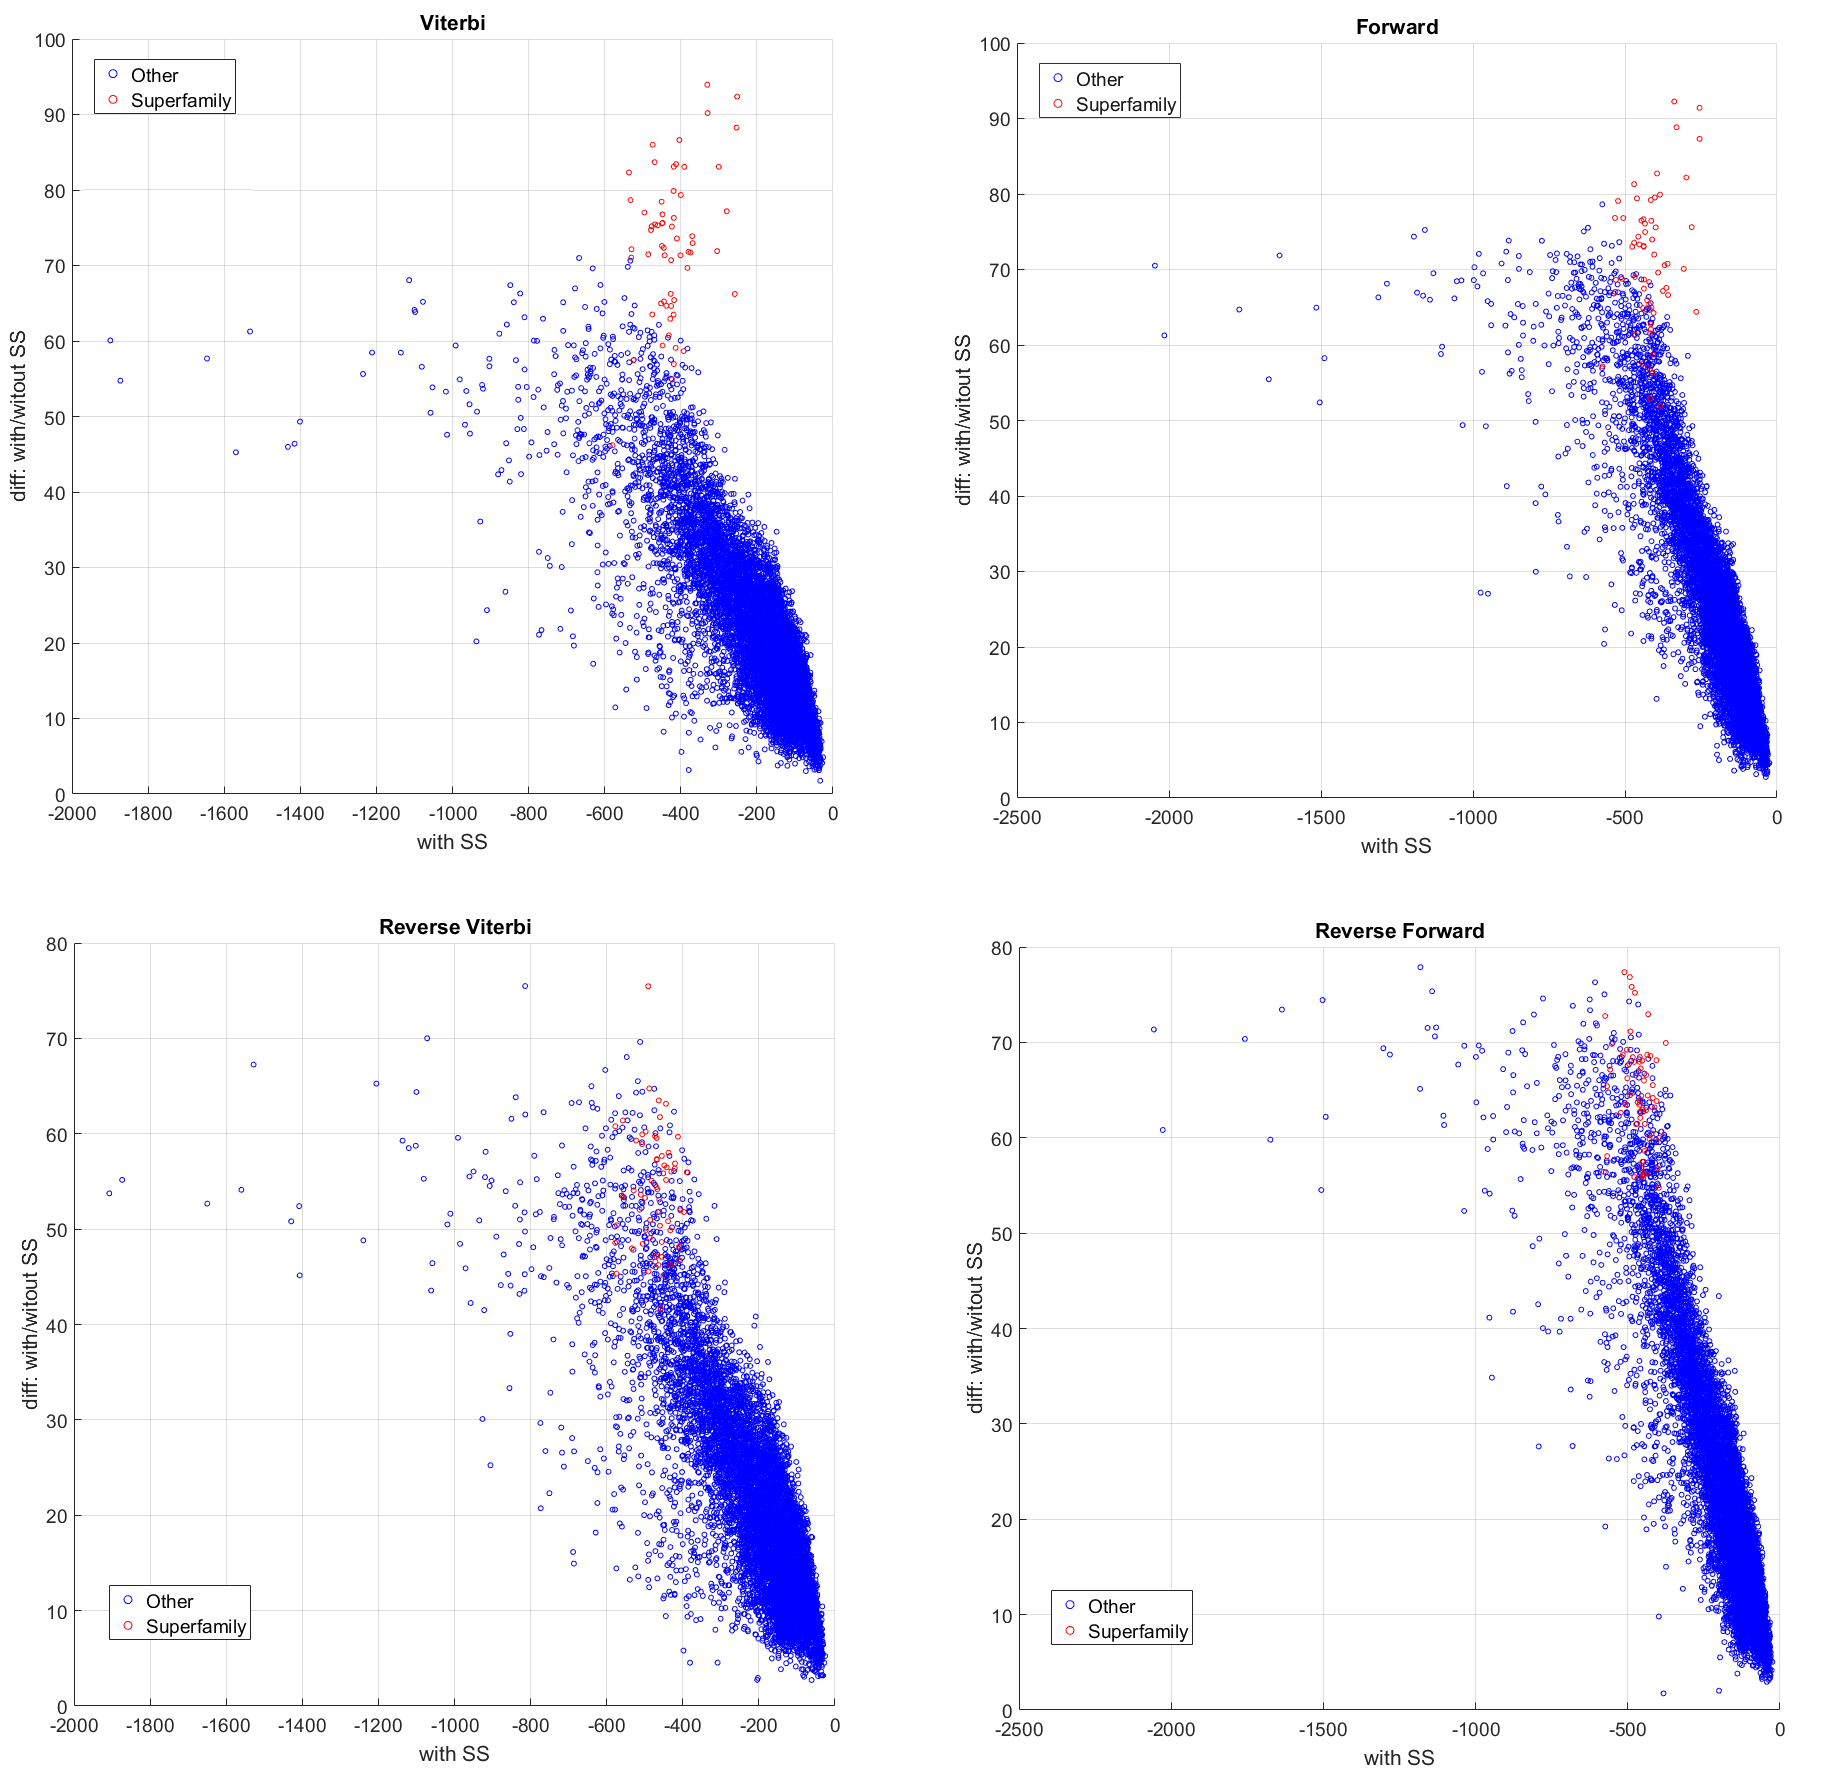
\includegraphics[width=0.97\textwidth]{fig/1plainUreversed}
	\end{center}
	\caption[Comparison between plain scores with and without secondary structure information.]{Comparison between plain scores with and without secondary structure information as scatterplots, with the score including secondary structure on the horizontal axis and on the vertical axis the difference from the scores with and without secondary structure information.}
	\label{fig:eval1}
\end{figure}


 


 
 
 
 %%%%%%%%%%%%%%%%
%%%%%  		Reverse corrected Scores
%%%%%%%%%%%%%%%
Figure \ref{fig:eval1_revCorr} shows the reverse-corrected scores. 
These are the combinations of the plain Viterbi and forward scores with their respective reversed scores in Figure \ref{fig:eval1}, displayed as a scatterplot of the scores with and without secondary structure information. The horizontal axis of the plot shows the original scores obtained using only the primary structure. The vertical axis gives the corresponding scores calculated by including the secondary structure. The red line straight through the origin assists in identifying the change in each score. Scores where the original score equals the new score are positioned on the red line. The farther away a score is from the zero line, the larger the change in the score between the two methods. Scores above the line indicate an increase; scores below the line mark a decrease in the score when including secondary structure information.  
A so-called \textit{rug plot} is included in the following figures. The rug plot is a one-dimensional representation of the data points projected along the axis. These rug plots are separated for scores from the superfamily, indicated as red ticks, and the other points, shown as blue ticks.  

 \begin{figure}[h!]
	\begin{center}
		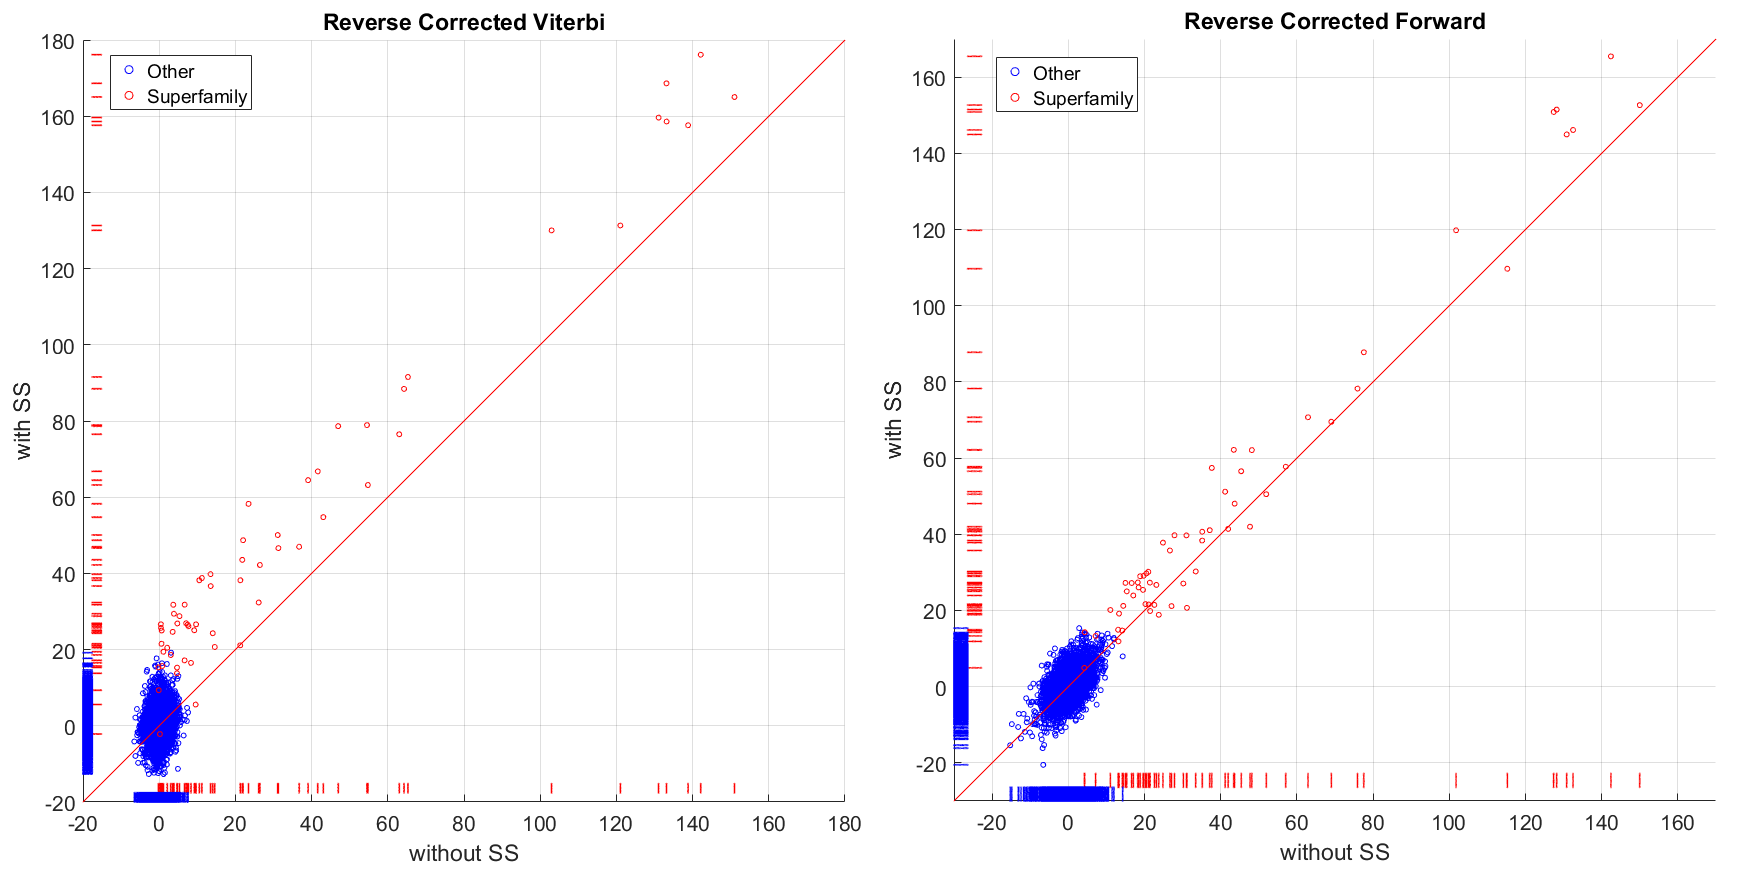
\includegraphics[width=0.99\textwidth]{fig/corr_4}
	\end{center}
	\caption[Scatterplots for comparing reverse-corrected scores with and without secondary structure information.]{Scatterplots for comparing reverse-corrected scores with and without secondary structure information on the horizontal axis and with secondary structure information in the vertical axis. }
	\label{fig:eval1_revCorr}
\end{figure}



Noticeable for the reverse-corrected Viterbi score is the dispersal of the other scores over twice the region when using secondary structure information. This difference is interesting due to its average change of below 0.5. However, except for three scores, the superfamily scores increase consistently. In particular, most superfamily scores close to zero and therefore surrounded by other scores increase more than the average and move away from the other scores. In contrast, the dispersal of the other scores for reverse-corrected forward scores remain closer to region of the original score. In addition, the rise of the superfamily scores is lower. While several low scores perform better than the other scores, there are also some decreasing superfamily scores.





Figure \ref{fig:eval1_simp} shows the same plot as Figure \ref{fig:eval1_revCorr}, but with the two simple-corrected scores. These are the simple null model scores subtracted from the plain Viterbi and forward scores. The simple null model uses the same general background distribution; therefore, there is no change when including secondary structure information. As a consequence, the region of all scores for the two simple-corrected scores increases according to the average score change listed in Table  \ref{tab:LST_Scores}. Moreover, except for a few outliers, the superfamily scores separate clearly from the other scores.


\begin{figure}[H]
	\begin{center}
		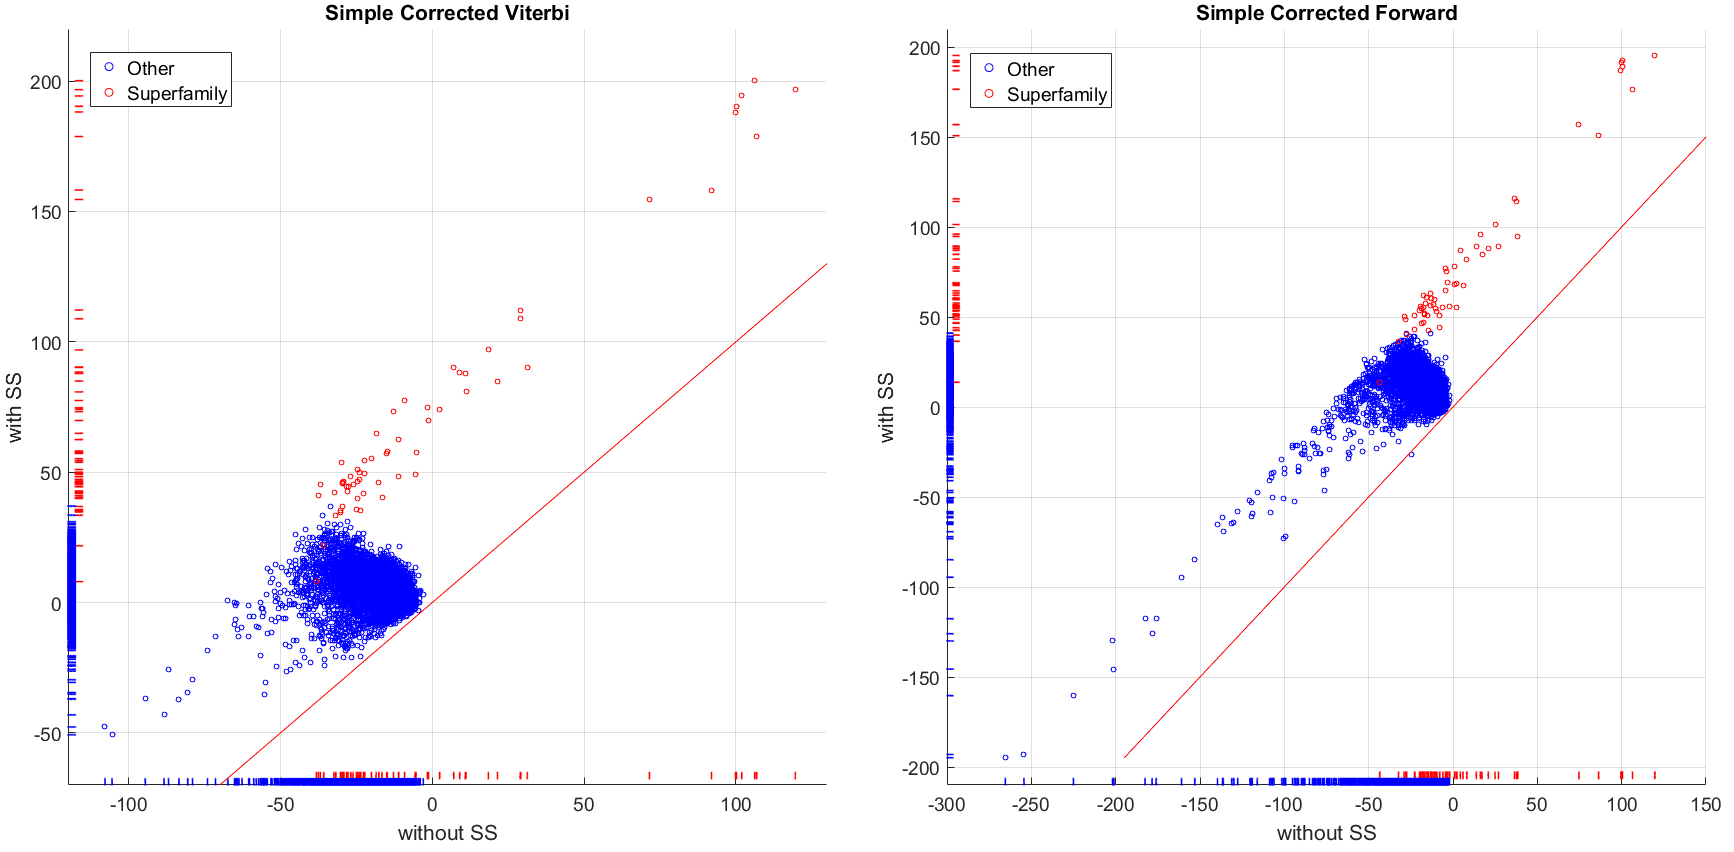
\includegraphics[width=0.92\textwidth]{fig/1simpleCorr}
	\end{center}
	\caption[Scatterplots for comparing simple-corrected scores with and without secondary structure information.]{Scatterplots for comparing simple-corrected scores with only the primary structure information on the horizontal axis with scores calculated using secondary structure information on the vertical axis. }
	\label{fig:eval1_simp}
\end{figure}
